\chapter{Process Modeling Notations and Agents}
\label{chapter:processes}

A possible reason for the slow uptake of agent concepts in industry is the gap that exists between the mentalistic notions used in agent theory and the business people's mindsets of services and processes.
The business world has been occupied by processes and web services. Thus the best way to establish agent technology and to close that gap seems to be providing a method to translate business process diagrams to agent systems.

The reason we decided for business process diagrams instead of UML is that we want to address the business people, which preferably use business processes, while UML is used mainly by the developers.

In the first section of this chapter we will briefly introduce JIAC, the main target language in the mapping to be described in this work. After that we will have a look on the various existing process modeling notations. We will explain why we picked BPMN as the source language for the transformation, comparing it with UML Activity Diagrams. Finally we will provide an overview on the most important elements and features of BPMN.



\section{Introducing JIAC}

The \emph{Java Intelligent Agent Componentware} (JIAC) is a framework for agent oriented software development. The Core of JIAC is the \emph{JIAC Agent Description Language} (JADL) \cite{konnerth05jadl}. The JIAC framework provides features such as FIPA compliant communication, Believe-Desire-Intention (BDI) reasoning, strong migration, web-service connectivity and others. Further it provides high security (\emph{Common Criteria EAL3}, certified by the Federal Office for Information Security of Germany, BSI) and advanced accounting mechanisms, making it suitable for the use in industrial and commercial applications. The JIAC framework comes with a runtime environment and a toolsuite for the creation of agents.

JIAC agents are knowledge-based and consist of dynamic components -- Facts, Rules, Goals, Plans and Services -- that can be exchanged at runtime (see figure \ref{fig:jiacmodel}).

\begin{figure}[htp]
	\centering
	\includegraphics[width=1\textwidth]{figures/process/jiac_meta.png}
	\caption{The JIAC metamodel}
	\label{fig:jiacmodel}
\end{figure}

Facts are instantiations of categories, defined in JADL ontologies, which make up the agents' shared vocabulary. They represent the agent's knowledge of the world and himself, his ``state of mind'' to say to, and are used for instance for reasoning.

% rules und reasoning
Rules and Goals are used to control the agents behavior. Rules make the agent react on changes in its environment, that is, its knowledge base. Using Goals, the agent, following the BDI paradigm, will autonomously select a Plan or Service to make its Goal come true.

% services und ontos mit JADL beschrieben
Plans and Services define what the agent can do. For their description JADL is used. Services are made up of Plans and normally have either a user and a provider side or only a provider. More sophisticated patterns, such as contract net, are possible, too. For the communication between the user and provider roles Speechacts are used. In most cases the planelements consist of a script, which is basically similar to other programs with the usual control-flow constructs, such as branching, loops, sequential, alternative and parallel execution. However, JADL provides a number of rare features, like using unification for both the evaluation of formulas and for making assignments to variables. JADL is based on a three valued predicate logic (with possible values \verb|true|, \verb|false| and \verb|unknown|) suitable for open-world problems in uncertain environments. Services and Plans are selected depending on their preconditions and effects.

Finally JIAC agents can be supplemented with Java components, so called AgentBeans. These components allow the agent to interact with the real world, e.g. by providing user interfaces or a robot control.

% aggregation von agenten aus agentenrollen, vordefinierte (management, mobility, etc.)
JIAC already comes with a set of predefined agentroles, which can be aggregated to agents. These agentroles provide functionality for knowledge access, reasoning, mobility, the management of groups of agents as a agent platform and many more.

The mapping which we will describe in this work will focus on plans and services.


%%%%%%%%%%%%%%%%%%%%%%%%%%%%%%%%%%%%%%%%%%%%%%%%%
\newpage
\section{A Survey of Process Modeling Notations}

\emph{Process Modeling Languages} (PMLs) provide a very abstract view on a program or process. The central point of PMLs is the modeling of control flow, including branching and parallelism, communication and activities. Unlike UML, data modeling and data flow are subordinated elements. Using an easily understandable notation PMLs are best suited for communicating process specifications throughout the whole software development process, from the stakeholders and domain experts to the software architects and developers.

While there are some textual PMLs, such as BPEL, most PMLs have a graphical notation, and most of these graphical notations are very similar: Activities, which normally are complex operations such as method or service calls, are represented by nodes, which are connected by arrows, representing the control flow and the exchange of messages.

With today's \emph{Model Driven Engineering} the process model can be used throughout all stages of software engineering, from requirements analysis to implementation (see figure \ref{fig:use_of_models}). Of course other models and diagrams will be needed, too, covering those issues that are not topic to process modeling. However, the process model should fit the needs of all parties involved in the software development process: From business users and domain experts over business analysts and architects to developers. The notation has to be simple and intuitively to understand, yet meaningful, formal and non-ambiguous. %In the best case the model can be used to generate executable code from it, or the model itself is executable.

\begin{figure}[htp]
	\centering
	\includegraphics[width=.75\textwidth]{figures/process/software_eng.png}
	\caption[Use of one PML throughout software engineering]{Use of one Process Modeling Language throughout all stages of software engineering}
	\label{fig:use_of_models}
\end{figure}

Currently there are many different process modeling languages available, some of which are standardized, and even more are proprietary. In this section we will have a look on some common workflow and process modeling notations. We will give a brief description of the language and state its pros and cons with respect to the problem to be solved in this thesis.


\subsection{Petri Nets}

% mathematische definition
Petri Nets have a very formal, mathematical grounding. Mathematically a Petri Net is a 5-Tuple
$PN = (P,T,F,W,M_0)$ with 
$P = \{ p_1,\cdots,p_n \}$ (Places), 
$T = \{ t_1,\cdots,t_m \}$ (Transitions), 
$F \subseteq (T \times P) \cup (P \times T)$ (Flow), 
$W : F \rightarrow \{1,2,\cdots \}$ (Weight) and 
$M_0 : P \rightarrow \{0,1,2,\cdots \}$ (Marking). Visually the Places are represented as cycles, Transitions as bars, Flow as arcs, Weight (if > 1) as labels on the arcs and the Marking as Tokens on the Places (see figure \ref{fig:petrinet} for a simple example). Beside this definition there are many other types and extensions of Petri Nets, from simple Elemental Petri Nets, where the Weight is 1 for each Flow and Places have a maximum capacity of one Token, to colored, timed or prioritized Petri Nets.

\begin{figure}[htp]
	\centering
	\includegraphics[width=.75\textwidth]{figures/process/petrinet.png}
	\caption{A simple producer-consumer petri net}
	\label{fig:petrinet}
\end{figure}

% bipartit, aktivierung und feuern, concurrency, parallelism
With $F \subseteq (T \times P) \cup (P \times T)$ a Petri Net is a bipartite graph, meaning that the flow control, the arcs, may only go from a Place to a Transition or vice versa, but neither from a Place to a Place nor from a Transition to a Transition.
A Transition is \emph{active} if on each Place before the Transition there are as many Tokens as the arc's Weight. When an active Transition \emph{fires} Tokens are moved from the Places before to the Places after the Transition, according to the arcs' weight. Thus concurrency can be modeled with Places having multiple outgoing arcs, while parallelism is modeled with Transactions having multiple outgoing arcs (analogue for merging and synchronization).

% stateful
Another particularity of Petri Nets is that they do not only model a process, but also the \emph{state} the process currently is in, represented by the Marking (the Tokens). For more detailed information about petri nets please refer to \cite{Murata89}.

% usage and restrictions
Petri Nets are well-established and used throughout workflow management and software design for analysis and validation of behavioral properties such as \emph{Liveness}, \emph{Reachability} and \emph{Boundedness}, for instance to detect and avoid possible deadlock situations.

But while Petri Nets can be used to model and analyze nearly everything from basic producer-consumer systems to multiprocessor systems their notation is very abstract and hard to understand, not only for non-experts. For the same reason it does not seem to be reasonable to use Petri Nets to generate executable programs from. Thus they would not be a good choice for a tool intended to facilitate the model driven creation of agents using business processes.


\subsection{UML Activity Diagrams}

\emph{UML Activity Diagrams} is one of the many diagram types used in the Unified Modeling Language (UML) \cite[Chapter 12]{spec_uml}, which clearly is the most popular modeling notation. Since software development is often accompanied by creating UML diagrams it might stand to reason to use UML Activity Diagrams for modeling business processes.

The semantics of Activity Diagrams have changed from UML 1.x to UML2. While in UML 1.x Activity Diagrams were very similar to State Diagrams they have now been enhanced with more possibilities for modeling parallelism and communication via asynchronous communication. However, Activity Diagrams lack the information given in the other UML diagrams, and modeling them all can be difficult and time-consuming, especially for small-scale enterprises.

The core elements used in most UML Activity Diagrams, like boxes, edges and diamonds, are easily to understand for all business users (see figure \ref{fig:uml-mail} for a simple example). However there are some rarely used, yet important elements which might be unfamiliar to non-experts, like interruptible regions, expansion regions and parameter pins, providing ways for modeling exception handling and user interaction or iteration of collections of input parameters or object flow and signals.

\begin{figure}[htp]
	\centering
	\includegraphics[width=.75\textwidth]{figures/process/umlac.png}
	\caption{E-mail example as UML Activity Diagram}
	\label{fig:uml-mail}
\end{figure}

The elements are very clear and can be drawn easily by hand. But many elements of UML Activity Diagrams look very similar or ambiguous, like activities with parameter pins and expansion regions, which could lead to some confusion among unexperienced modelers.


\subsection{Business Process Modeling Notation}
\label{sec:bpmn_short}

%einführung
The \emph{Business Process Modeling Notation} was first published by the BPMI
% in 2004 
and has later been adopted by the OMG. The goal of the development of BPMN was to create a standardized modeling notation for business processes and by that to reduce the confusion created by dozens of proprietary business process notations. The BPMN is intended to ``consolidate the best ideas from these divergent notations into a single standard notation'' \cite[p. 9]{white04}.

% grundbausteine
There are four basic categories of element types in the notation: Flow Objects (Events, Activities  and Gateways), Connecting Objects (Sequence Flows, Message Flows and Associations), Swimlanes (Pools and Lanes) and Artifacts (Data Objects, Groups and Annotations). Please refer to section \ref{sec:bpmn} for more detailed information about the several elements.

\begin{figure}[htp]
	\centering
	\includegraphics[width=.75\textwidth]{figures/process/bpmn_mail.png}
	\caption{E-mail example in Business Process Modeling Notation}
	\label{fig:bpmn-mail}
\end{figure}

% basis-elemente and subtypes
Figure \ref{fig:bpmn-mail} shows a simple example for an e-mail client periodically looking for new mail. The elements are quite self-descriptive and most of them are already known from other notations, so the basics of the BPMN are readily understandable for all business analysts, architects and developers and even for non-experts. At the same time BPMN provides a large variety of subtypes for each of the Flow Objects and every element type is enriched with many non-graphical attributes, making the models sufficiently detailed for being exported to executable languages while keeping the visual notation concise and understandable.

A problem with BPMN is that it is mainly a \emph{notation}. Although the specification describes many non-graphical attributes and a mapping to a formal language, it neither states an exchange format, like an XSD, nor clear semantics for all of the elements. Still the Business Process Modeling Notation can be used throughout the whole software engineering lifecycle, from a simplified model at the requirements analysis up to a highly detailed model that can be used for generating code for an executable language.


\subsection{XPDL}

The \emph{XML Process Definition Language} (XPDL) \cite{spec_xpdl} is a workflow model interchange language standardized by the Workflow Management Coalition (WfMC). XPDL does not have a graphical notation on its own. Instead the goal of XPDL was to be an interface, a ``lingua franca'' \cite{ce-xpdl}, for the various diverging workflow notations and tools. In the beginning XPDL defined only a minimum set of core elements, but later many vendor specific extensions, including a large part of BPMN, have been adopted to XPDL, making the specification very large and hard to overview: The XPDL's XML Schema Definition is about 110kB in size, compared to 25kB in the case of BPEL.

An evaluation of XPDL with respect to its expressiveness when modeling a number of workflow patterns \cite{ce-xpdl} was rather disillusioning. It seemed that the expressiveness of XPDL was ``the intersection rather than the union'' of that of other workflow notations. Being used as an interchange language the modeler would have to constrain his diagrams to those elements supported by XPDL (and, in case XPDL offers more than a given notation, it would not be possible to transfer an XPDL diagram to this notation).

In its latest version XPDL is intended to be the syntactical counterpart to the graphical notations defined by BPMN. While the idea behind XPDL clearly is ambitious it suffers from a inflated notation and complicated syntax.


\subsection{Simple Notation}
%  erste abschnitte beziehen die benutzer mit ein -> benutzer müssen die notation auch verstehen
In a thought experiment Havey \cite{havey} states that even a notation like BPMN might not be simple enough to be understood by most business users. While it might be possible for them to understand most of a diagram drawn using BPMN they wouldn't be able to modify or create one on their own. There are too many details, such as constraints and restrictions on the use of some elements in certain situations, which are not obvious on first sight, so having the business users participating in drawing such a diagram would need too much guidance by the professionals.

% einführung simple notation
Havey proposes to use a \emph{Simple Notation} for the requirements analysis, which is very intuitive to understand. Machines, on the other hand, won't be able to understand this notation, thus the models will have to be translated to a more formal notation later on.

% beschreibung simple notation
The Simple Notation is made up of only four elements: Boxes and arrows for the concepts of activities and control flow. Further there are annotations (which are represented as plain boxes, too) and associations, e.g. to bind an annotation to a node. There are no restrictions on how to label the nodes and edges, since everything will be intuitively to understand by humans. See figure \ref{fig:simple-mail} for how the e-mail example from earlier in this section could look in Simple Notation.

\begin{figure}[htp]
	\centering
	\includegraphics[width=.75\textwidth]{figures/process/simple_mail.png}
	\caption{E-mail example in Simple Notation}
	\label{fig:simple-mail}
\end{figure}

% mächtigkeit der sprache
These few elements are enough to model the basic workflow patterns such as decisions and loops. However, for modeling more complex situations like reacting on events or more sophisticated control flow rich use of annotations will be necessary, making diagrams drawn in the Simple Notation intuitively but weary to understand. Further some diagrams might be ambiguous and not clear to understand by other readers -- let alone machines.


\subsection{Proprietary Notations}
Many modeling tools for the Business Process Execution Language (BPEL) provide their own graphical notation for BPEL. Making use of the fact that most elements of BPEL are block-structured the resulting diagrams often look like a mixture of BPMN and Nassi-Shneiderman diagrams. While these diagrams are of course very close to the executable code, making it easy for BPEL experts to write and maintain processes, it is obvious that this type of diagram is not suited for exchange among different departments and institutions.



\section{Comparing BPMN and UML Activity Diagrams}

% activity diagrams werden oft sowieso erstellt
From the above, UML Activity Diagrams and BPMN obviously are the best choices. Both are standardized, formal and not too difficult to understand. But while creating models using UML has taken its place in the software development lifecycle BPMN still is a new technique. In this section we will compare these two notations.

White \cite{bpmnVsAct} compared BPMN and UML Activity Diagrams by testing their capability of describing 21 workflow patterns\footnote{meanwhile the list has been extended to 43 patterns, see \cite{patterns2}}\cite{patterns1}. Most of these patterns can be drawn nearly equally with both notations, but while in BPMN often there are several possibilities of drawing a certain pattern Activity Diagrams are more restrictive. He explains the similarity of both notations with the fact that both are designed to describe the same domain. He writes that they even might ``converge'' some day. The first step, the adoption of BPMN by the OMG, is already done.

UML is a very large specification with many different diagrams, each showing only one view on the model. Each diagram has its own notation and rules. Elements, such as arrows of some line style, have different meanings in different diagrams of UML. In BPMN there is only one type of diagram providing one view on the system, but this one view is more complex, providing more information than UML Activity Diagrams. With BPMN being used instead of UML Activity Diagrams the process models will be more precise. BPMN will never replace UML, but it is a good addition.

% bpmn allein reicht nicht, uml für datenmodellierung, dennoch bpmn besser geeignet für prozessmodellierung als activity diagrams
While UML is the more \emph{complete} modeling notation BPMN has the advantage that all the information is caught in a \emph{single} diagram. BPMN is not suited for modeling data structures and data flow, but for processes it's more powerful than UML Activity Diagrams.

With its subtypes and attributes a diagram written in BPMN is providing more information than a similar UML Activity Diagram. This information can be used for a mapping (and thus for exporting) to a executable language. Depending on how accurate the model can be mapped to the target language, the mapping could be rough, regarding the basic types only, or very accurate, finding an equivalent for each attribute and diagram pattern, thus BPMN diagrams could be mapped to instantly executable programs.

% fazit: simple -> bpmn -> executable
The best choice for the requirements analysis might be to use a simplified version of the BPMN, with only the basic elements and some simple to understand subtypes such as timer events or standard loops, or to change to a more simplified notation in case the business users show too few understanding. In both cases the process model will have to be refined or even redrawn by the professionals after the requirements analysis. From this point on it can be used throughout the further design. After the design phase it can be transformed to an executable language, being the fundament for the final implementation.


\section{A Closer Look at BPMN}
\label{sec:bpmn}

% intro
After the short introduction earlier in this chapter we will use this section to take a closer look at BPMN, since this will be the process modeling language used in this thesis. More details and advanced modeling techniques can be found in the full specification \cite{spec_bpmn}.


\subsection{BPMN Elements}

This section is intended to give a brief introduction of each of the basic element groups:

\begin{itemize}
	\item \textbf{Flow Objects}: Events (Start, End and Intermediate), Activities (Task and Subprocess) and Gateways
	\item \textbf{Connecting Objects}: Sequence Flows, Message Flows and Associations
	\item \textbf{Swimlanes}: Pools and Lanes
	\item \textbf{Artifacts}: Data Objects, Groups and Annotations
\end{itemize}

\subsubsection*{Flow Objects}

The category of \emph{Flow Objects}, the most important elements in BPMN, is made up of \emph{Events}, \emph{Activities} and \emph{Gateways}. All Flow Objects are held in Lanes (see below).

\textbf{Events} are things that \emph{happen}, like a message arriving, an alarm, or an error, and often they mark the beginning and the end of the process. The graphical notation is a circle. They are subdivided into \emph{Start Events}, \emph{Intermediate Events} and \emph{End Events}, which will determine the circle's border (see figure \ref{fig:events}).

\begin{figure}[htp]
	\centering
	
\includegraphics[width=.75\textwidth]{figures/bpmn/events.png}
	\caption[BPMN Event types]{BPMN Event types. From left to right: Start Event, Intermediate Event, End Event}
	\label{fig:events}
\end{figure}

Further all three Event types have a variety of subtypes which will determine e.g. a Start Event's \emph{trigger} and an end Event's \emph{result}. Each of these subtypes can be distinguished by a different icon in the center of the Event figure (see figure \ref{fig:triggers}) and results in a number of attributes to be set for the Event.

\begin{figure}[htp]
	\centering
	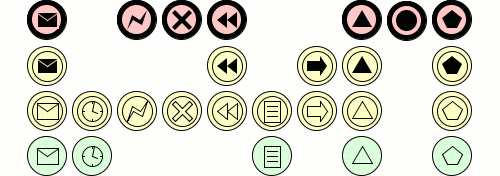
\includegraphics[width=.75\textwidth]{figures/bpmn/triggers.png}
	\caption[BPMN Event sub types]{BPMN Event sub types. From left to right: Rule, Timer, Message, Link, Multiple, Cancel, Compensate, Error, Terminate}
	\label{fig:triggers}
\end{figure}

Basically, an \textbf{Activity} is something that is \emph{done}. Activities subdivide in \emph{Tasks}, which are atomic Activities, and \emph{Subprocesses}, which are composite Activities. The graphical notation for an Activity is a rounded rectangle with the Activity's name inside of it. Subprocesses are marked with a small $ \boxplus $ sign on the bottom line (see figure \ref{fig:activities}).

\begin{figure}[htp]
	\centering
	
\includegraphics[width=.75\textwidth]{figures/bpmn/activities.png}
	\caption[BPMN Activity types]{BPMN Activity types. From left to right: Task, Subprocess}
	\label{fig:activities}
\end{figure}

Like Events, Activities also have some specializations, each one with special attributes: They can be for instance a \emph{Send} or a \emph{Receive} Task, stand for some \emph{Manual} work to be done, execute a \emph{Script} or, in case of the \emph{Independent} Subprocess, represent a whole business process, just to name a few. All of these subtypes have the same graphical representation, but modelers and modeling tools are free to extend the diagrams with additional markers for the subtypes.

What makes Activities stand out from the other Flow Objects is that they can \emph{loop}. Although in BPMN loops also can be defined by simply connecting a Sequence Flow to an upstream Flow Object, which might be easier to understand by non-experts, it's seen as better style to use looping Subprocesses. A looping Activity is marked with a small counter-clockwise arrow on its bottom line.

\textbf{Gateways} provide wide capabilities in modeling all kinds of splitting and merging behavior. Figure \ref{fig:gateways} shown the different kinds of Gateways. Depending on whether the Gateway has multiple incoming or outgoing Sequence Flows -- or even both -- it has different semantics, like forking and/or joining the flows. However, Gateways are not the only way for modeling forking and joining of flows. In some cases the same semantics can be reached by omitting the Gateway and connecting multiple Sequence Flows directly to an Activity\footnote{this is not allowed for Events}.

\begin{figure}[htp]
	\centering
	
\includegraphics[width=.75\textwidth]{figures/bpmn/gateways.png}
	\caption[BPMN Gateway types]{BPMN Gateway types. From left to right: Data based XOR (with and without marker), Event based XOR, Inclusive OR, Complex, AND}
	\label{fig:gateways}
\end{figure}

\subsubsection*{Connecting Objects}

The most important connections are \emph{Sequence Flows} and \emph{Message Flows}. Sequence Flows represent the flow of control and connect Flow Objects within a Pool in the order of execution. Message Flow represents messages -- not necessarily data -- being exchanged exclusively between Pools. See figure \ref{fig:connections} for the connections' graphical notation.

\begin{figure}[htp]
	\centering
	
\includegraphics[width=.75\textwidth]{figures/bpmn/connections.png}
	\caption[BPMN Connection types]{BPMN Connection types. From left to right: Sequence Flow, Message Flow, Association}
	\label{fig:connections}
\end{figure}

The third connection, the \emph{Association}, is mainly used for documentation reason, for instance to connect a Text Annotation to a Flow Object that needs further explanation. Still there is an exceptions to this rule: For connecting a compensating Activity to a compensation Event an Association is used instead of a Sequence Flow. An Association's arrow heads are optional.

\subsubsection*{Swimlanes}

Swimlanes can be \emph{Pools} and \emph{Lanes}. Each Pool represents one Participant in the business process, while Lanes are used to partition a Pool. Doing so each of a company's departments could be represented by a Lane while the Pool stands for the company itself. Typically Pools and Lanes are oriented horizontally, but they may be oriented vertically, too. Further, Lanes may cross or contain other Lanes, but those techniques are poorly documented and usually not used. Figure \ref{fig:swimlanes} shows a small horizontally oriented Pool containing two empty Lanes.

\begin{figure}[htp]
	\centering
	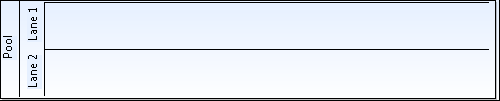
\includegraphics[width=.75\textwidth]{figures/bpmn/swimlanes.png}
	\caption[BPMN Swimlanes]{BPMN Swimlanes. A Pool with two Lanes}
	\label{fig:swimlanes}
\end{figure}

\subsubsection*{Artifacts}

The main purpose of \emph{Artifacts} is documentation. However, like Associations, in some situations they can have semantics, e.g. when a \emph{Data Object} is referenced by an Activity as input. Data Objects represent everything that can be input or output of some Activity. In most cases this will be a file, but since Activities can be \emph{Manual Tasks}, too, a Data Object could also stand for something physical.

The other two Artifacts, \emph{Group} and \emph{Text Annotation}, are solely used for documentation. See figure \ref{fig:artifacts} for their graphical notation.

\begin{figure}[htp]
	\centering
	
\includegraphics[width=.75\textwidth]{figures/bpmn/artifacts.png}
	\caption[BPMN Artifacts]{BPMN Artifacts. From left to right: Data Object, Group, Text Annotation}
	\label{fig:artifacts}
\end{figure}

The specification states that this category may be extended by proprietary artifacts which could have more semantics, too. This way BPMN can be extended with new elements to represent concepts that were not considered in the original specification.


\subsection{Levels of Complexity}

% drei layer
BPMN can be seen as having at least three levels of complexity.

\begin{enumerate}
	\item Basic Types: All diagrams are made up of the basic elements of the four categories: Events, Activities, Gateways, Connections, Pools and Artifacts. These can be understood easily even by non-experts.
	\item Subtypes: The Flow Objects each have several subtypes, e.g. Timer Events, Receive Tasks and Inclusive Gateways. Using the same shapes as the basic elements enriched with some additional graphical information, like an icon, the symbol's basic type can be clearly identified by non-experts while providing additional visual information for the professionals.
	\item Attributes: Each of the BPMN element types provides a large number of both primitive and complex attributes. While some of these attributes are visible in the diagram, like a flow object's name or subtype, most are non-graphical. These attributes enrich the diagram with the formal semantics necessary for the export to an executable language while not polluting the visual notation with too many details.
\end{enumerate}

% notation teils ohne semantik (message flows)
If the process shall be mapped to a executable language the third level is very important: Not only does it give values for many attributes that otherwise would have to be set manually. Some of the visual elements of the BPMN do not have semantics ``on their own''. Message Flows for example do \emph{not} have a mapping to WS-BPEL. Instead the source Activity has to be of type \verb|Send| and the target Activity of type \verb|Receive|, and both have to reference the same non-graphical \verb|Message| element. This is necessary in cases when the communications partner is not in the same diagram and thus a Message Flow can not be drawn.

Of course it is free to the designers of new mappings to map the Message Flow, if it is available, without insisting on the existence of the non-graphical Message element.


\subsection{Export and Code Generation}

One of the main purposes of the Business Process Modeling Notation is to provide a graphical notation that can be used to generate executable code from it.

A mapping to WS-BPEL is given in the BPMN Specification \cite[Chapter 11]{spec_bpmn}. As a matter of fact the BPMN has been tailored for the mapping to WS-BPEL, which can be seen in many attributes which are needed only for the mapping. Most of these attributes can be reused for mappings to other languages, too, e.g. such common concepts as properties and assignments.

On the other side BPMN has more expressive power than BPEL. A diagram in BPMN is a directed graph, while BPEL (and in fact most other executive languages as well) is block oriented, making the export to a semantically equivalent program somewhat complicated and in some cases impossible. Numerous papers have been written on how to identify block structures within a BPMN diagram or how to alter an existing diagram to conform to block structure. However, not every diagram can be refactored like that.

While the basic elements such as Flow Objects shall neither be altered nor extended by new elements the BPMN Specification encourages the introduction of new, domain-specific Artifacts to be used in mappings to executable languages other than BPEL. These elements can be associated with the original BPMN elements and represent concepts that were not considered in the original BPMN specification.
\\
\\

In this chapter a number of process modeling notations have been introduced and the core elements and features of the Business Process Modeling Notation have been lined out. The next chapter will briefly introduce the basic concepts of Model Driven Engineering and how they can be applied for generating powerful domain specific editors. Further an overview on known problems and existing approaches concerning the model driven generation of executable programs based on process models will be given.
